\documentclass{../common/SCNU_Experimental_Report}

% 填写报告头信息
\studentname{汤承洲}
\studentid{20233902058}
\major{电子信息工程}
\class{23级2班}
\coursename{控制工程}
\projectname{PID控制器的设计}
\verify
\experimentdate{2026年6月9日}
\teacher{熊爱民}

\graphicspath{{./figures/}}

\begin{document}
\maketitle

\section{实验目的}
\begin{enumerate}
    \item 研究PID控制器中比例系数\(K_p\)、积分时间常数\(T_i\)和微分时间常数\(T_d\)对闭环系统阶跃响应的影响。
    \item 掌握Ziegler-Nichols（齐格勒-尼科尔斯）工程整定方法，能够对典型被控对象进行PID参数整定。
    \item 学会在MATLAB环境中使用PID控制器进行系统仿真，并通过性能指标（上升时间、超调量、调节时间等）评估控制效果。
\end{enumerate}

\section{实验原理}
\subsection{模拟PID控制器}

典型的PID控制结构如图~\ref{fig:pid_struct}所示。输入信号\(r(t)\)与反馈信号\(y(t)\)通过求和节点产生误差信号\(e(t)\)。误差信号分为三路，分别进入比例、积分、微分三个环节，其输出相加得到控制信号\(u(t)\)，作用于被控对象产生系统输出\(y(t)\)，输出通过负反馈回路送回输入端。

\begin{figure}[H]
    \centering
    % PID控制结构框图（原图片文件缺失，已移除，以文字描述替代）
    \caption{PID控制结构框图}
    \label{fig:pid_struct}
\end{figure}

PID调节器的数学描述为：
\[
u(t) = K_p \left[ e(t) + \frac{1}{T_i}\int_0^t e(\tau)d\tau + T_d\frac{de(t)}{dt} \right]
\]

其中，\(K_p\)为比例系数，\(T_i\)为积分时间常数，\(T_d\)为微分时间常数。比例环节即时响应误差，积分环节消除稳态误差，微分环节预测误差变化趋势并增加系统阻尼。

\subsection{数字PID控制器}

在计算机控制中，连续PID算法需经离散化处理。以一阶后向差分近似微分、矩形法数值积分近似积分：
\[
\begin{cases}
t \approx kT \\
\displaystyle\int_0^t e(\tau)d\tau \approx T\sum_{j=0}^{k} e(j) \\
\displaystyle\frac{de(t)}{dt} \approx \frac{e(k) - e(k-1)}{T}
\end{cases}
\]

离散PID表达式为：
\[
u(k) = K_p \left[ e(k) + \frac{T}{T_i}\sum_{j=0}^{k} e(j) + \frac{T_d}{T}\left(e(k) - e(k-1)\right) \right]
\]

其中\(T\)为采样周期。

\subsection{Ziegler-Nichols整定法}

Ziegler-Nichols法是经典的PID参数工程整定方法。对于稳定的被控对象，先令\(T_i \to \infty\)、\(T_d = 0\)，仅使用比例控制，逐步增大\(K_p\)直至系统输出产生等幅振荡，记录此时的临界增益\(K_c\)和临界振荡周期\(T_c\)。然后按下表计算PID参数：

\begin{table}[H]
    \centering
    \caption{Ziegler-Nichols PID参数整定公式}
    \label{tab:zn}
    \small
    \begin{tabular}{cccc}
        \toprule
        控制器类型 & \(K_p\) & \(T_i\) & \(T_d\) \\
        \midrule
        P & \(0.5 K_c\) & \(\infty\) & 0 \\
        PI & \(0.45 K_c\) & \(0.85 T_c\) & 0 \\
        PID & \(0.6 K_c\) & \(0.5 T_c\) & \(0.125 T_c\) \\
        \bottomrule
    \end{tabular}
\end{table}

\section{实验内容}

本次实验以三阶对象\(G(s) = 1/(s+1)^3\)为被控对象，分为两个任务：任务一研究PID参数对闭环系统阶跃响应的影响；任务二使用Ziegler-Nichols法进行PID参数整定并优化。

\subsection{任务一：PID参数对闭环系统阶跃响应的影响}

被控对象为三阶系统：
\[
G(s) = \frac{1}{(s+1)^3}
\]

\subsubsection{(1) 纯比例控制：不同\(K_p\)值下的阶跃响应（\(T_i \to \infty\)，\(T_d \to 0\)）}

在\(T_i \to \infty\)、\(T_d \to 0\)的条件下，系统退化为纯比例控制。取\(K_p = 0.5, 1, 2, 3, 4, 5\)，观察闭环系统的阶跃响应变化。

\begin{figure}[H]
    \centering
    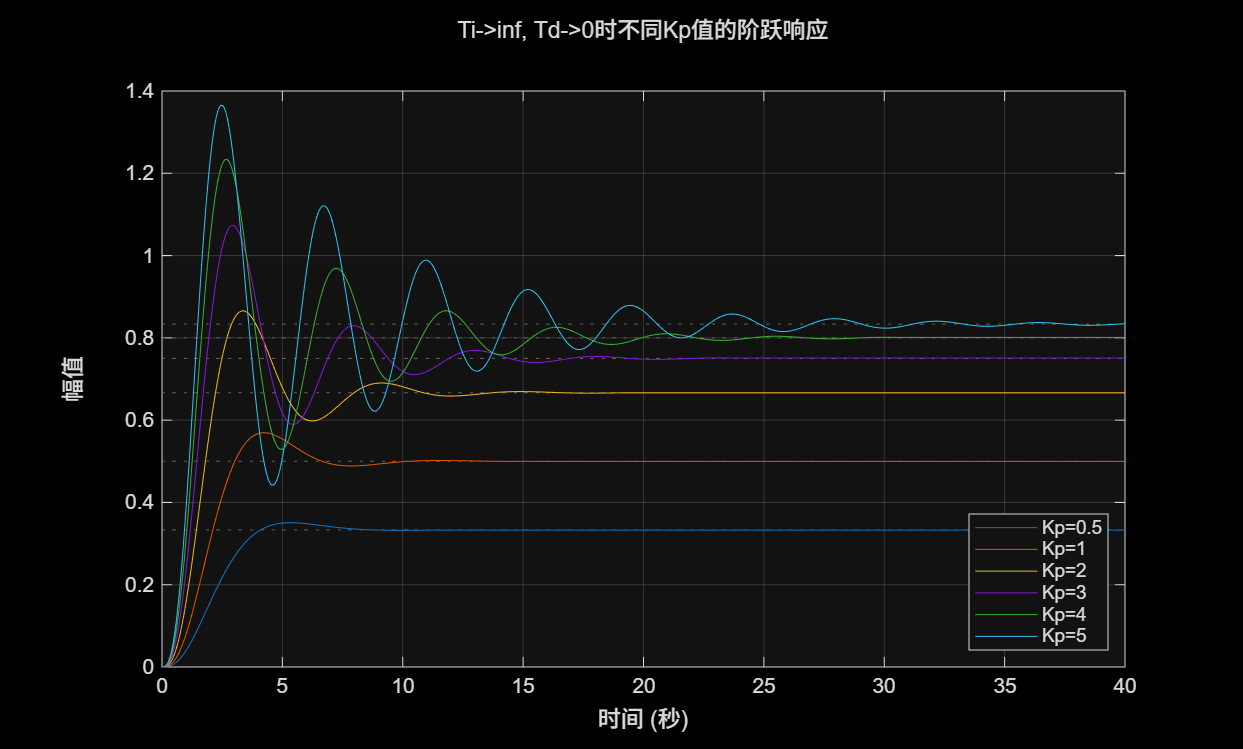
\includegraphics[width=0.75\textwidth]{./figures/Task01_Figure_1.png}
    \caption{不同\(K_p\)值下的阶跃响应（\(T_i \to \infty\)，\(T_d \to 0\)）}
    \label{fig:ex6_task1_kp}
\end{figure}

\textbf{结果分析：}随着\(K_p\)增大，系统响应加快（上升时间缩短），但超调量逐渐增大。\(K_p = 0.5\)时响应缓慢且无超调；\(K_p = 3\)时出现明显超调；\(K_p = 5\)时超调显著增大，系统趋于临界不稳定状态。纯比例控制存在稳态误差，且过大的\(K_p\)会恶化系统稳定性。

\subsubsection{(2) PI控制：不同\(T_i\)值下的阶跃响应（\(K_p = 1\)，\(T_d \to 0\)）}

固定\(K_p = 1\)、\(T_d \to 0\)，取\(T_i = 0.5, 1, 2, 5, 10\)，分析积分时间常数对系统响应的影响。根据极点分布判断稳定性，将稳定与不稳定的曲线分别绘制。

\begin{figure}[H]
    \centering
    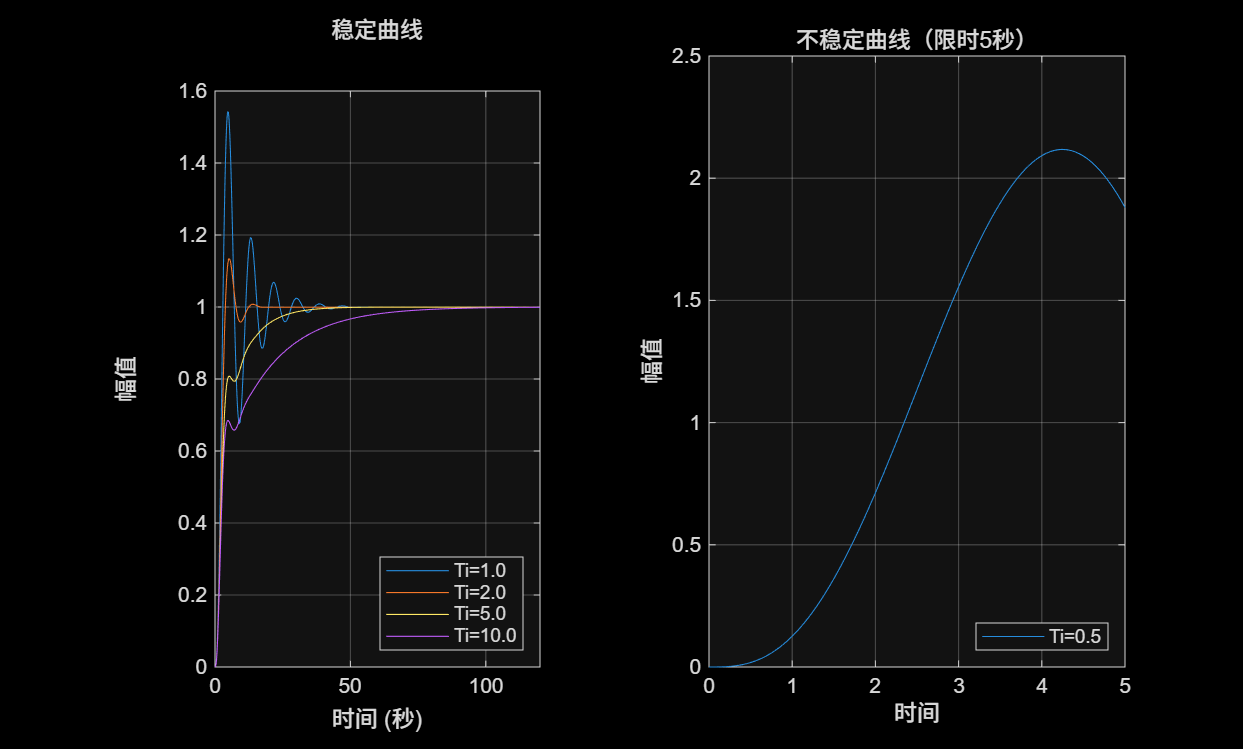
\includegraphics[width=0.85\textwidth]{./figures/Task01_Figure_2.png}
    \caption{不同\(T_i\)值下的阶跃响应（\(K_p = 1\)，\(T_d \to 0\)）：(左) 稳定曲线 (右) 不稳定曲线}
    \label{fig:ex6_task1_ti}
\end{figure}

\textbf{结果分析：}当\(T_i = 0.5\)时，极点位于右半平面，系统发散不稳定；当\(T_i \geq 1\)时系统稳定。在同一\(K_p\)下，\(T_i\)越小积分作用越强，稳态误差消除越快，但系统稳定性变差；\(T_i\)越大积分作用越弱，响应曲线趋向于纯比例控制的效果。积分环节的引入能够消除稳态误差，但会降低系统的稳定性裕度。

\subsubsection{(3) PID控制：不同\(T_d\)值下的阶跃响应（\(K_p = T_i = 1\)）}

固定\(K_p = 1\)、\(T_i = 1\)，取\(T_d = 0, 0.5, 1, 2, 3, 4\)，分析微分时间常数对系统响应的影响。

\begin{figure}[H]
    \centering
    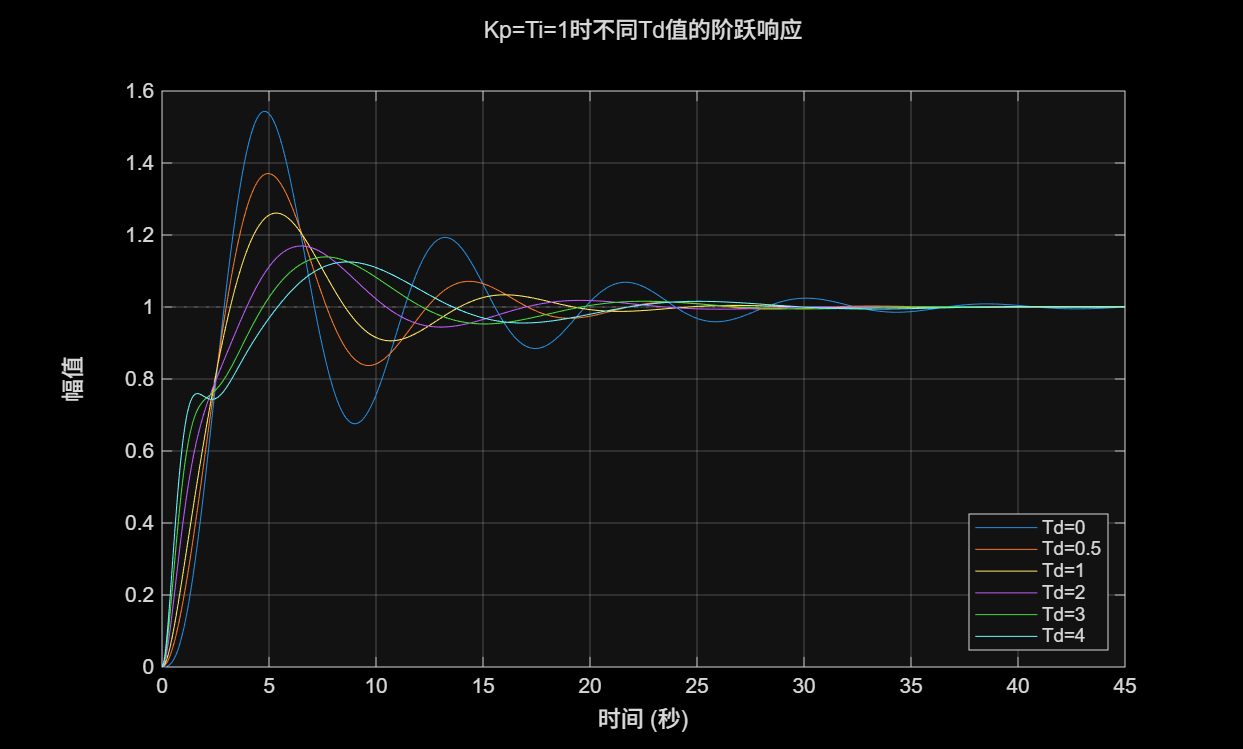
\includegraphics[width=0.75\textwidth]{./figures/Task01_Figure_3.png}
    \caption{不同\(T_d\)值下的阶跃响应（\(K_p = T_i = 1\)）}
    \label{fig:ex6_task1_td}
\end{figure}

\textbf{结果分析：}随着\(T_d\)增大，微分作用增强，系统阻尼增加，超调量显著减小，响应曲线趋于平缓。\(T_d = 0\)时系统超调最大；\(T_d = 0.5 \sim 1\)时超调明显减小，响应速度和阻尼达到较好的平衡；\(T_d = 3 \sim 4\)时响应虽然平滑但上升时间明显延长。说明适当的微分作用可改善系统阻尼特性，但过大的微分会降低响应速度。

\subsection{任务二：PID参数整定（Ziegler-Nichols法）}

\subsubsection{系统的根轨迹分析}

首先绘制被控对象\(G(s) = 1/(s+1)^3\)的根轨迹图，分析系统的稳定性特征。

\begin{figure}[H]
    \centering
    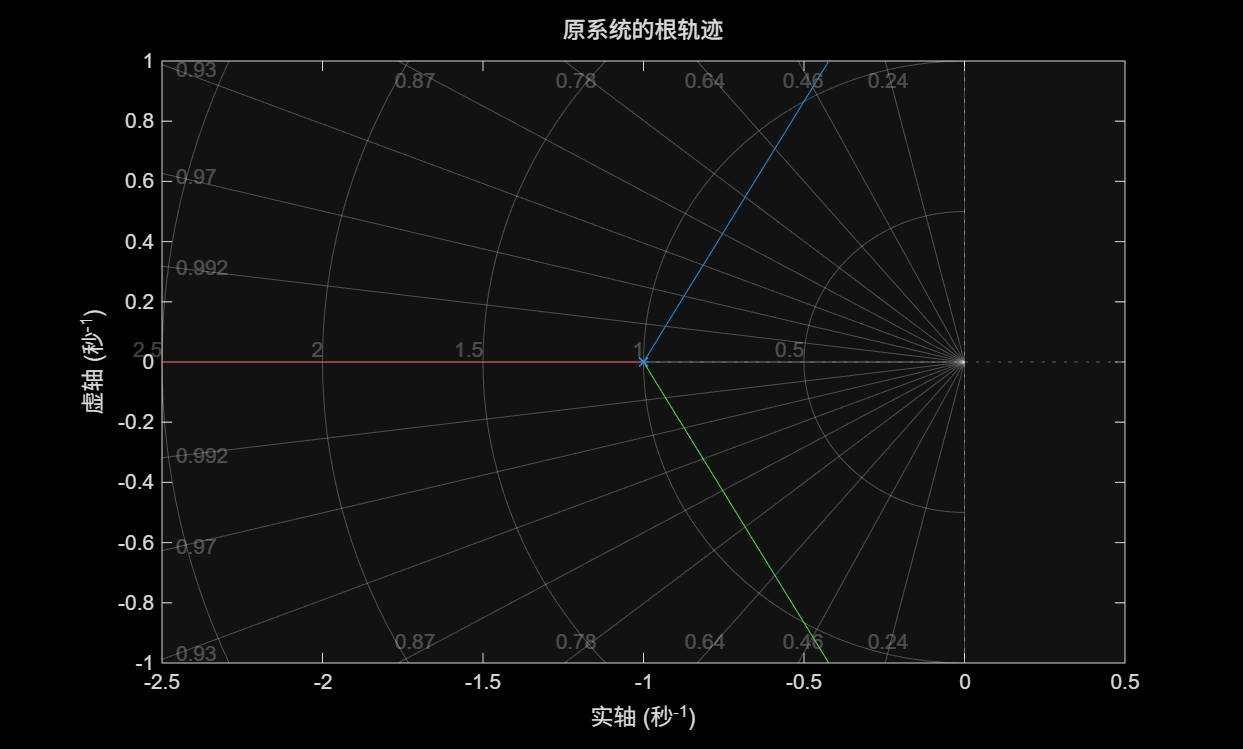
\includegraphics[width=0.75\textwidth]{./figures/Task02_Figure_1.png}
    \caption{原系统的根轨迹图}
    \label{fig:ex6_task2_rlocus}
\end{figure}

对于三阶对象\(G(s)=1/(s+1)^3\)，手动计算得到临界参数：
\[
K_c = 8, \quad T_c = \frac{2\pi}{\sqrt{3}} \approx 3.6276 \text{ s}
\]

\subsubsection{Ziegler-Nichols PID参数整定}

根据Z-N整定公式计算PID参数：
\begin{align*}
K_p &= 0.6 K_c = 4.8000 \\
T_i &= 0.5 T_c = 1.8138 \\
T_d &= 0.125 T_c = 0.4534
\end{align*}

使用整定后的PID控制器进行阶跃响应仿真：

\begin{figure}[H]
    \centering
    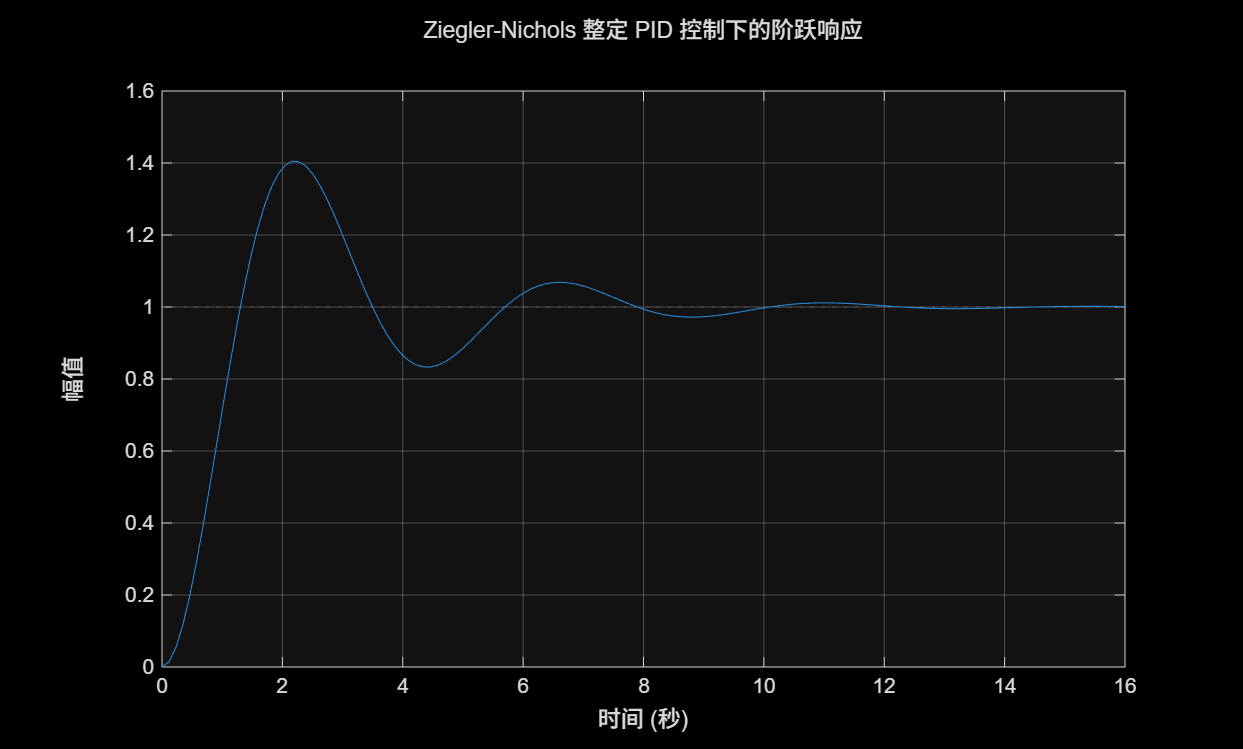
\includegraphics[width=0.75\textwidth]{./figures/Task02_Figure_2.png}
    \caption{Ziegler-Nichols整定PID控制下的阶跃响应}
    \label{fig:ex6_task2_zn}
\end{figure}

\subsubsection{参数微调与性能对比}

在Z-N参数基础上进行微调：\(K_p\)降至\(3.8400\)（\(0.8 K_{p\_zn}\)），\(T_i\)降至\(1.6324\)（\(0.9 T_{i\_zn}\)），\(T_d\)增至\(0.5441\)（\(1.2 T_{d\_zn}\)）。

\begin{figure}[H]
    \centering
    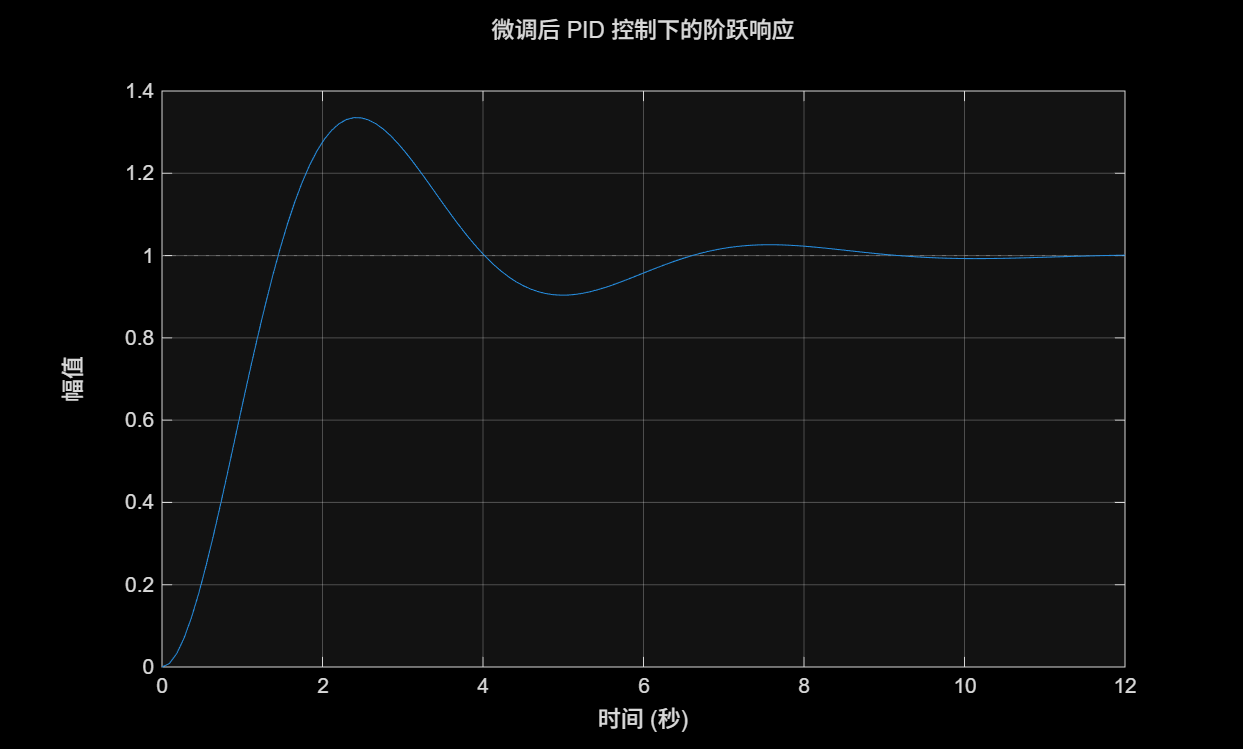
\includegraphics[width=0.75\textwidth]{./figures/Task02_Figure_3.png}
    \caption{微调后PID控制下的阶跃响应}
    \label{fig:ex6_task2_tuned}
\end{figure}

性能指标对比如下：

\begin{table}[H]
    \centering
    \caption{Z-N PID与微调后PID性能指标对比}
    \label{tab:perf_compare}
    \small
    \begin{tabular}{cccc}
        \toprule
        指标 & Z-N PID & 微调后PID & 变化趋势 \\
        \midrule
        上升时间(s) & 0.8761 & 0.9831 & 略有增加 \\
        峰值时间(s) & 2.1641 & 2.3904 & 略有增加 \\
        超调量(\%) & 40.49 & 33.52 & 显著减小 \\
        调节时间(s) & 9.3721 & 8.1661 & 明显缩短 \\
        \bottomrule
    \end{tabular}
\end{table}

\textbf{结果分析：}微调后的PID虽然上升时间略有增加（从0.8761s增至0.9831s），但超调量从40.49\%降至33.52\%，调节时间从9.3721s缩短至8.1661s，综合性能优于Z-N整定参数。这表明适当降低\(K_p\)和\(T_i\)、增大\(T_d\)可以在抑制超调与缩短调节时间之间取得更好的平衡。

\subsubsection{PID各参数影响的进一步分析}

固定其他参数为Z-N整定值，分别改变\(K_p\)、\(T_i\)、\(T_d\)，观察各参数对系统响应的影响。

\begin{figure}[H]
    \centering
    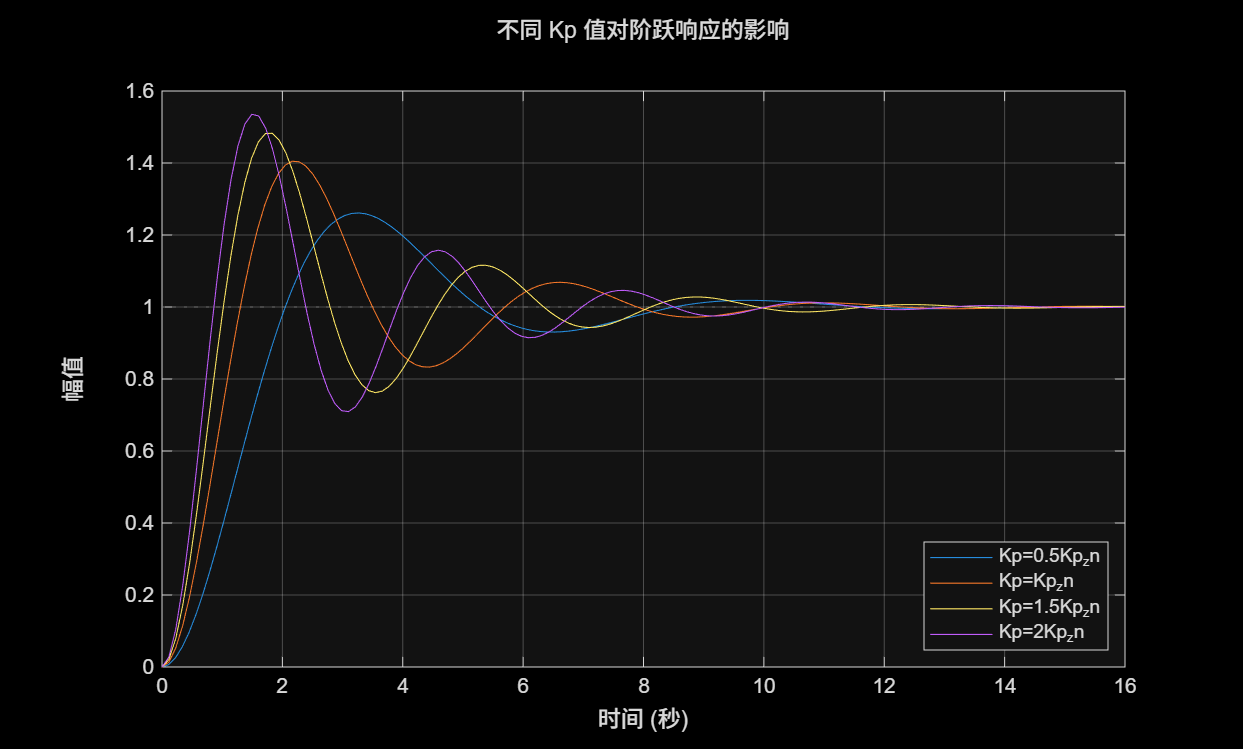
\includegraphics[width=0.75\textwidth]{./figures/Task02_Figure_4.png}
    \caption{不同\(K_p\)值对阶跃响应的影响}
    \label{fig:ex6_task2_kp_effect}
\end{figure}

\begin{figure}[H]
    \centering
    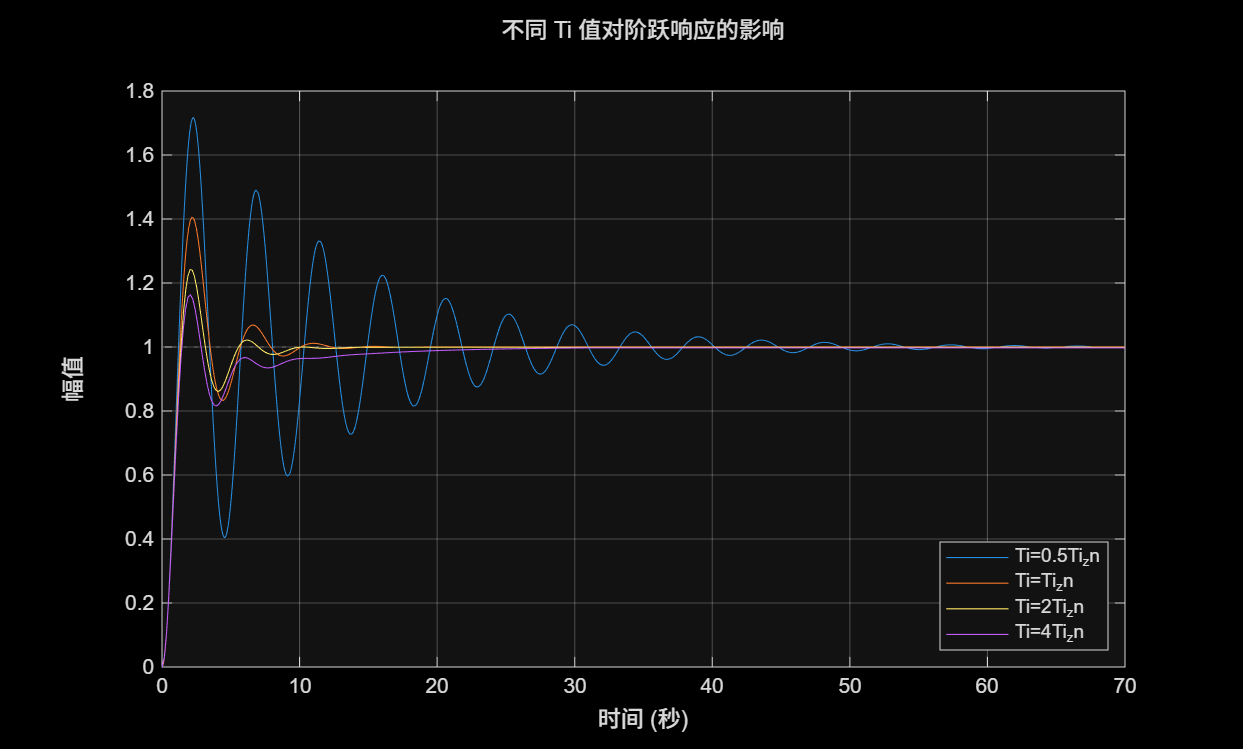
\includegraphics[width=0.75\textwidth]{./figures/Task02_Figure_5.png}
    \caption{不同\(T_i\)值对阶跃响应的影响}
    \label{fig:ex6_task2_ti_effect}
\end{figure}

\begin{figure}[H]
    \centering
    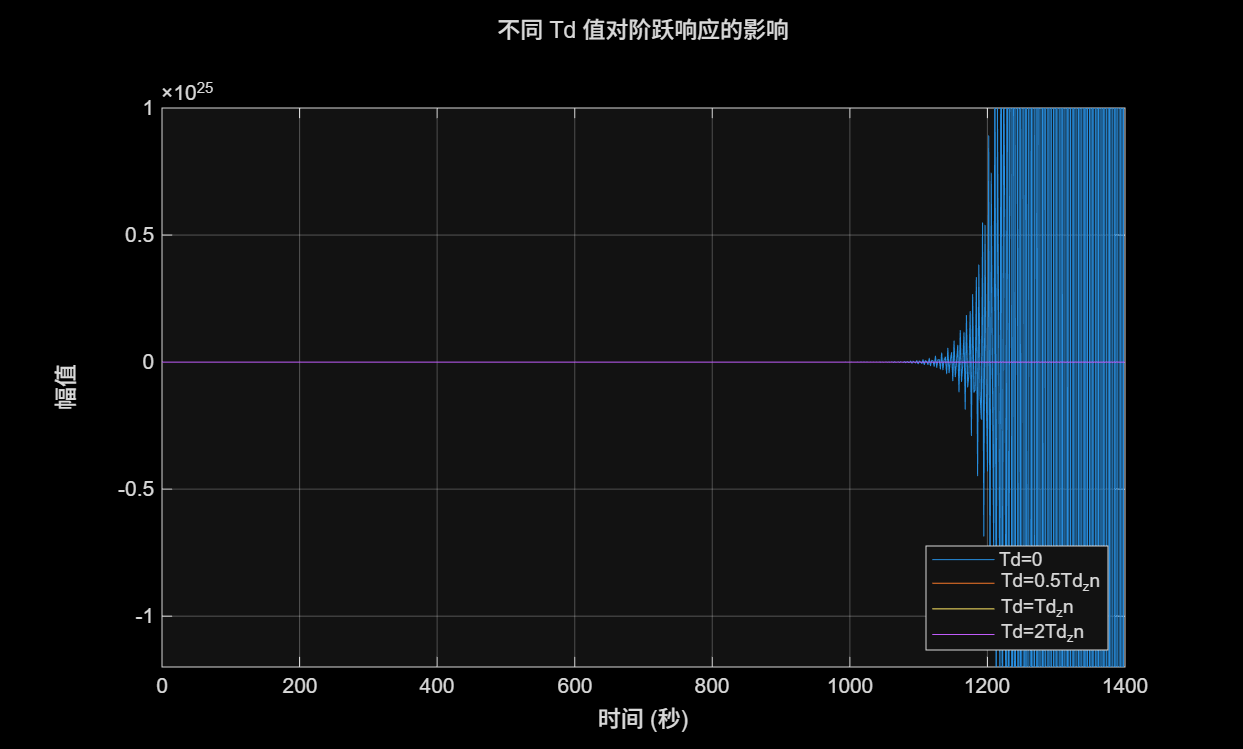
\includegraphics[width=0.75\textwidth]{./figures/Task02_Figure_6.png}
    \caption{不同\(T_d\)值对阶跃响应的影响}
    \label{fig:ex6_task2_td_effect}
\end{figure}

\textbf{结果分析：}
\begin{itemize}
    \item \textbf{\(K_p\)的影响：}增大\(K_p\)使响应加快、上升时间缩短，但超调量增大，系统稳定性降低。\(K_p = 2K_{p\_zn}\)时系统出现明显的振荡。
    \item \textbf{\(T_i\)的影响：}减小\(T_i\)增强积分作用，加快稳态误差消除，但超调增大、稳定性下降；增大\(T_i\)使响应趋近于纯比例控制，稳态误差消除变慢。
    \item \textbf{\(T_d\)的影响：}增大\(T_d\)增强微分阻尼作用，超调量减小，系统稳定性改善，但过大的\(T_d\)会显著降低响应速度。
\end{itemize}

\subsubsection{最优参数选择}

综合权衡各项性能指标，选取最优参数\(K_p = 3.3600\)（\(0.7 K_{p\_zn}\)）、\(T_i = 1.4510\)（\(0.8 T_{i\_zn}\)）、\(T_d = 0.4534\)（\(1.0 T_{d\_zn}\)）。

\begin{figure}[H]
    \centering
    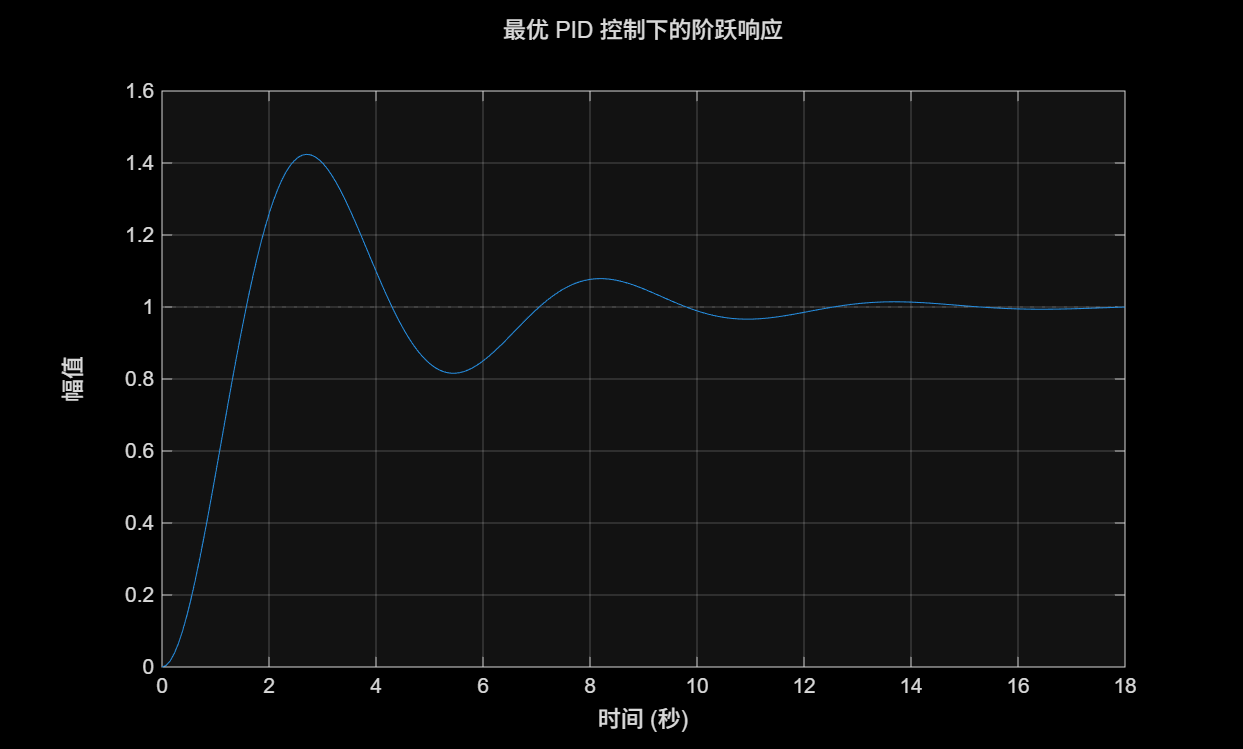
\includegraphics[width=0.75\textwidth]{./figures/Task02_Figure_7.png}
    \caption{最优PID控制下的阶跃响应}
    \label{fig:ex6_task2_opt}
\end{figure}

最优PID参数性能：
\begin{itemize}
    \item 上升时间：1.0593 s
    \item 超调量：42.41\%
    \item 调节时间：11.8093 s
\end{itemize}

\textbf{结果分析：}相比微调参数，最优参数进一步降低了\(K_p\)和\(T_i\)，响应更加平稳但上升时间和调节时间变长。说明PID参数整定需要在快速性（上升时间）和稳定性（超调量、调节时间）之间进行折中，不存在使所有指标同时最优的单一参数组合。

\section{实验总结}

本次实验系统地研究了PID控制器参数对闭环系统动态性能的影响，并掌握了Ziegler-Nichols工程整定方法，主要收获如下：

\subsection{PID参数影响规律}
\begin{enumerate}
    \item \textbf{比例系数\(K_p\)：}增大\(K_p\)可加快响应速度、缩短上升时间，但会增大超调量、降低系统稳定性。过大的\(K_p\)可能导致系统不稳定。
    \item \textbf{积分时间常数\(T_i\)：}减小\(T_i\)增强积分作用，有利于消除稳态误差，但会增大超调、降低稳定性。当\(T_i\)过小时系统可能出现不稳定（如本次实验中\(T_i = 0.5\)时系统发散）。
    \item \textbf{微分时间常数\(T_d\)：}增大\(T_d\)增强微分阻尼，可有效抑制超调，改善系统稳定性，但过大的\(T_d\)会降低响应速度。
\end{enumerate}

\subsection{Ziegler-Nichols整定方法}
\begin{enumerate}
    \item Z-N法通过临界增益\(K_c\)和临界振荡周期\(T_c\)快速获取PID参数初值：\(K_p = 4.8000\)、\(T_i = 1.8138\)、\(T_d = 0.4534\)，所得系统上升时间快（0.8761s）但超调偏高（40.49\%）。
    \item 在Z-N参数基础上进行微调（降低\(K_p\)和\(T_i\)、增大\(T_d\)），可将超调量降至33.52\%，调节时间缩短至8.1661s，综合性能优于原始Z-N参数。
    \item 最优参数选择需在快速性与稳定性之间折中：进一步降低\(K_p\)和\(T_i\)虽能提高稳定性，但会牺牲响应速度。
\end{enumerate}

\subsection{实验心得}
通过本次实验，加深了对PID控制器各参数物理意义的理解，掌握了利用MATLAB进行控制系统仿真的方法，以及通过时域性能指标（上升时间、超调量、调节时间等）定量评估控制效果的技能。Ziegler-Nichols法提供了良好的参数初值，实际工程中还需结合具体指标要求进行微调优化，以达到最佳的控制性能。

\section{实验源码}

\subsection{task1.m：PID参数对闭环系统阶跃响应的影响}
\begin{lstlisting}[language=Matlab]
% task1 研究闭环系统在不同控制情况下的阶跃响应
clc;
clear;
close all;
diary('results/logs/Task01_output.log');

% 三阶对象模型 G(s) = 1 / (s + 1)^3
s = tf('s');
G = 1 / (s + 1)^3;

%% 1. Ti -> inf, Td -> 0 时, 在不同 Kp 值下, 闭环系统的阶跃响应
figure;

Kp_list = [0.5, 1, 2, 3, 4, 5];
for i = 1:length(Kp_list)
    Kp = Kp_list(i);
    % 纯比例控制：Ti = inf, Td = 0, N = Inf
    C = pidstd(Kp, Inf, 0, Inf);
    G_cl = feedback(C * G, 1);
    step(G_cl);
    hold on;
end

legend('Kp=0.5', 'Kp=1', 'Kp=2', 'Kp=3', 'Kp=4', 'Kp=5', 'Location', 'southeast');
title('Ti->inf, Td->0时不同Kp值的阶跃响应');
xlabel('时间');
ylabel('幅值');
grid on;
hold off;
saveas(gcf, 'results/figures/Task01_Figure_1.png');

%% 2. Kp = 1, Td -> 0 时，在不同 Ti 值下, 闭环系统的阶跃响应
Ti_list = [0.5, 1, 2, 5, 10];

% 判断稳定性，分组合并
stable_Ti = [];
unstable_Ti = [];

for i = 1:length(Ti_list)
    Ti = Ti_list(i);
    C = pidstd(1, Ti, 0, Inf);
    G_cl = feedback(C * G, 1);
    poles = pole(G_cl);
    if all(real(poles) < 0)
        stable_Ti = [stable_Ti, Ti];
    else
        unstable_Ti = [unstable_Ti, Ti];
    end
end

% 子图1：稳定的曲线
figure;
subplot(1, 2, 1);
for i = 1:length(stable_Ti)
    Ti = stable_Ti(i);
    C = pidstd(1, Ti, 0, Inf);
    G_cl = feedback(C * G, 1);
    step(G_cl);
    hold on;
end
legend(arrayfun(@(x) sprintf('Ti=%.1f', x), stable_Ti, 'UniformOutput', false), ...
    'Location', 'southeast');
title('稳定曲线');
xlabel('时间');
ylabel('幅值');
grid on;
hold off;

% 子图2：不稳定的曲线（限时5秒）
subplot(1, 2, 2);
for i = 1:length(unstable_Ti)
    Ti = unstable_Ti(i);
    C = pidstd(1, Ti, 0, Inf);
    G_cl = feedback(C * G, 1);
    [y, t] = step(G_cl, 5);
    plot(t, y);
    hold on;
end
legend(arrayfun(@(x) sprintf('Ti=%.1f', x), unstable_Ti, 'UniformOutput', false), ...
    'Location', 'southeast');
title('不稳定曲线（限时5秒）');
xlabel('时间');
ylabel('幅值');
grid on;
hold off;
saveas(gcf, 'results/figures/Task01_Figure_2.png');

%% 3. Kp = Ti = 1 时, 在不同 Td 值下, 闭环系统的阶跃响应
figure;

Td_list = [0, 0.5, 1, 2, 3, 4];
for i = 1:length(Td_list)
    Td = Td_list(i);
    C = pidstd(1, 1, Td, Inf);
    G_cl = feedback(C * G, 1);
    step(G_cl);
    hold on;
end

legend('Td=0', 'Td=0.5', 'Td=1', 'Td=2', 'Td=3', 'Td=4', 'Location', 'southeast');
title('Kp=Ti=1时不同Td值的阶跃响应');
xlabel('时间');
ylabel('幅值');
grid on;
hold off;
saveas(gcf, 'results/figures/Task01_Figure_3.png');

diary off;
\end{lstlisting}

\subsection{task2.m：PID参数整定（Ziegler-Nichols法）}
\begin{lstlisting}[language=Matlab]
% task2 选择合适的参数进行模拟 PID 控制
clc;
clear;
close all;
diary('results/logs/Task02_output.log');

% 三阶对象模型 G(s) = 1 / (s + 1)^3
s = tf('s');
G = 1 / (s + 1)^3;

% 手动计算临界增益（对于 G(s)=1/(s+1)^3）
Kc = 8;
Tc = 2 * pi / sqrt(3);  % ≈ 3.6276

fprintf('临界增益 Kc = %.4f\n', Kc);
fprintf('临界振荡周期 Tc = %.4f 秒\n', Tc);

% Ziegler-Nichols PID 参数（标准型）
Kp_zn = 0.6 * Kc;
Ti_zn = 0.5 * Tc;
Td_zn = 0.125 * Tc;

fprintf('\nZiegler-Nichols 整定参数:\n');
fprintf('Kp = %.4f\n', Kp_zn);
fprintf('Ti = %.4f\n', Ti_zn);
fprintf('Td = %.4f\n', Td_zn);

%% 1. 根轨迹图
figure;
rlocus(G);
title('原系统的根轨迹');
grid on;
saveas(gcf, 'results/figures/Task02_Figure_1.png');

%% 2. 使用整定后的 PID 控制器进行仿真
figure;

C_zn = pidstd(Kp_zn, Ti_zn, Td_zn, Inf);
G_cl_zn = feedback(C_zn * G, 1);
step(G_cl_zn);
grid on;
title('Ziegler-Nichols 整定 PID 控制下的阶跃响应');
xlabel('时间');
ylabel('幅值');
saveas(gcf, 'results/figures/Task02_Figure_2.png');

%% 3. 微调参数以获得更好的响应
figure;

Kp_tune = Kp_zn * 0.8;
Ti_tune = Ti_zn * 0.9;
Td_tune = Td_zn * 1.2;

C_tune = pidstd(Kp_tune, Ti_tune, Td_tune, Inf);
G_cl_tune = feedback(C_tune * G, 1);
step(G_cl_tune);
grid on;
title('微调后 PID 控制下的阶跃响应');
xlabel('时间');
ylabel('幅值');
saveas(gcf, 'results/figures/Task02_Figure_3.png');

%% 4. 性能指标对比
info_zn = stepinfo(G_cl_zn);
info_tune = stepinfo(G_cl_tune);

fprintf('\n性能指标对比:\n');
fprintf('指标\t\tZ-N PID\t\t微调后 PID\n');
fprintf('上升时间(s)\t%.4f\t\t%.4f\n', info_zn.RiseTime, info_tune.RiseTime);
fprintf('峰值时间(s)\t%.4f\t\t%.4f\n', info_zn.PeakTime, info_tune.PeakTime);
fprintf('超调量(%%)\t%.2f\t\t%.2f\n', info_zn.Overshoot, info_tune.Overshoot);
fprintf('调节时间(s)\t%.4f\t\t%.4f\n', info_zn.SettlingTime, info_tune.SettlingTime);

%% 5. 分析不同 PID 参数的影响
% (1) 不同 Kp 值的影响
figure;

Kp_test = [Kp_zn * 0.5, Kp_zn, Kp_zn * 1.5, Kp_zn * 2];
for i = 1:length(Kp_test)
    C_test = pidstd(Kp_test(i), Ti_zn, Td_zn, Inf);
    G_cl_test = feedback(C_test * G, 1);
    step(G_cl_test);
    hold on;
end

legend('Kp=0.5Kp_zn', 'Kp=Kp_zn', 'Kp=1.5Kp_zn', 'Kp=2Kp_zn', ...
    'Location', 'southeast');
title('不同 Kp 值对阶跃响应的影响');
xlabel('时间');
ylabel('幅值');
grid on;
hold off;
saveas(gcf, 'results/figures/Task02_Figure_4.png');

% (2) 不同 Ti 值的影响
figure;

Ti_test = [Ti_zn * 0.5, Ti_zn, Ti_zn * 2, Ti_zn * 4];
for i = 1:length(Ti_test)
    C_test = pidstd(Kp_zn, Ti_test(i), Td_zn, Inf);
    G_cl_test = feedback(C_test * G, 1);
    step(G_cl_test);
    hold on;
end

legend('Ti=0.5Ti_zn', 'Ti=Ti_zn', 'Ti=2Ti_zn', 'Ti=4Ti_zn', ...
    'Location', 'southeast');
title('不同 Ti 值对阶跃响应的影响');
xlabel('时间');
ylabel('幅值');
grid on;
hold off;
saveas(gcf, 'results/figures/Task02_Figure_5.png');

% (3) 不同 Td 值的影响
figure;

Td_test = [0, Td_zn * 0.5, Td_zn, Td_zn * 2];
for i = 1:length(Td_test)
    C_test = pidstd(Kp_zn, Ti_zn, Td_test(i), Inf);
    G_cl_test = feedback(C_test * G, 1);
    step(G_cl_test);
    hold on;
end

legend('Td=0', 'Td=0.5Td_zn', 'Td=Td_zn', 'Td=2Td_zn', ...
    'Location', 'southeast');
title('不同 Td 值对阶跃响应的影响');
xlabel('时间');
ylabel('幅值');
grid on;
hold off;
saveas(gcf, 'results/figures/Task02_Figure_6.png');

%% 6. 选择最优参数并显示最终响应
figure;

Kp_opt = Kp_zn * 0.7;
Ti_opt = Ti_zn * 0.8;
Td_opt = Td_zn * 1.0;

C_opt = pidstd(Kp_opt, Ti_opt, Td_opt, Inf);
G_cl_opt = feedback(C_opt * G, 1);
step(G_cl_opt);
grid on;
title('最优 PID 控制下的阶跃响应');
xlabel('时间');
ylabel('幅值');
saveas(gcf, 'results/figures/Task02_Figure_7.png');

info_opt = stepinfo(G_cl_opt);
fprintf('\n最优 PID 参数及性能:\n');
fprintf('Kp = %.4f, Ti = %.4f, Td = %.4f\n', Kp_opt, Ti_opt, Td_opt);
fprintf('上升时间 = %.4f\n', info_opt.RiseTime);
fprintf('超调量 = %.2f %%\n', info_opt.Overshoot);
fprintf('调节时间 = %.4f\n', info_opt.SettlingTime);

diary off;
\end{lstlisting}

\end{document}
